% ARC S2 Engineer arm: product summary. Build: python -I cad/docs/paper/make_paper.py
% Every number is a macro from numbers.tex, which make_paper.py writes from the check results.
% Pictures: fig/render_*.png from cad/render (blender -b -P cad/render/blender_render.py -- --stills);
%           fig/sim_*.png from cad/sim/tasks.py --snap;
%           fig/build_*.png: FreeCAD GUI views from cad/render/build_steps.py (after cad/tools/build_guide.py, which also writes build/*.tex).
\documentclass[10pt]{article}
\usepackage[margin=1in]{geometry}
\usepackage{lmodern}
\usepackage[T1]{fontenc}
\usepackage{amsmath,amssymb}
\usepackage{graphicx}
\usepackage{booktabs}
\usepackage{caption}
\usepackage{subcaption}
\usepackage{microtype}
\usepackage[hidelinks]{hyperref}
\usepackage[section]{placeins}
\captionsetup{font=small,labelfont=bf}
\renewcommand{\topfraction}{0.9}\renewcommand{\bottomfraction}{0.8}\renewcommand{\textfraction}{0.07}\renewcommand{\floatpagefraction}{0.8}
% generated by make_paper.py from the check results; do not edit
\newcommand{\ArmMass}{1266}
\newcommand{\ArmMassDirect}{1350}
\newcommand{\PastWrist}{567}
\newcommand{\HeadMass}{356}
\newcommand{\JOneTau}{3.40}
\newcommand{\JTwoTau}{2.92}
\newcommand{\JThreeTau}{0.88}
\newcommand{\JOneUtilG}{81}
\newcommand{\JTwoUtilG}{70}
\newcommand{\JOneUtilD}{38}
\newcommand{\JTwoUtilD}{32}
\newcommand{\JThreeUtil}{60}
\newcommand{\HoldSTS}{4.19}
\newcommand{\HoldDM}{9.0}
\newcommand{\Ratio}{3}
\newcommand{\DonutRated}{1.74}
\newcommand{\DonutStall}{6.0}
\newcommand{\PipeRated}{1.13}
\newcommand{\PipeStall}{5.6}
\newcommand{\MinSF}{1.8}
\newcommand{\MinSFPart}{Link LD lo CF3}
\newcommand{\SimTime}{85.6}
\newcommand{\PeakFrac}{47}
\newcommand{\RmsFrac}{90}
\newcommand{\DeadPoint}{24.7}
\newcommand{\Overlaps}{0}
\newcommand{\PipeDepth}{297}
\newcommand{\ReleaseTime}{0.04}
\newcommand{\DirectExtra}{85}
\newcommand{\JOneOverRated}{22}
\newcommand{\FusionVerB}{23}
\newcommand{\FusionMassB}{2024}
\newcommand{\FusionTqDiffB}{5}
\newcommand{\FusionVerA}{24}
\newcommand{\FusionMassA}{2169}
\newcommand{\FusionTqDiffA}{5}
\newcommand{\FusionSolids}{526}

% generated by cad/tools/build_guide.py: one \buildstep{key} body per step; do not edit
\expandafter\def\csname buildstep@base\endcsname{%
\begin{center}\render{build_01_base.jpg}{0.62\linewidth}\\[-2pt]{\footnotesize Step 1: Base frame. Orange: added in this step; blue: bench sub-assembly mounted; grey: already built.}\end{center}
\paragraph{Parts.}
\begin{center}\footnotesize\begin{tabular}{@{}p{0.30\linewidth}rp{0.58\linewidth}@{}}\toprule
Part & Qty & Prototype / description \\ \midrule
Base\_Plate\_AL5 & 1 & print; production: 5 mm 6061, waterjet + tap \\
Tower\_Bracket\_L & 2 & print; production: PETG-CF print \\
Tower\_Bracket\_R & 2 & print; production: PETG-CF print \\
Tower\_L\_CF3 & 1 & print; production: 3 mm CF plate (DXF) \\
Tower\_R\_CF3 & 1 & print; production: 3 mm CF plate (DXF) \\
BHCS M3x10 & 4 & ISO 7380 button head screw \\
BHCS M3x8 & 4 & ISO 7380 button head screw \\
CLIP & 2 & Adhesive cable-tie mount 10x10 + 2.5 mm cable tie \\
Nyloc M3 & 4 & ISO 10511 nyloc nut \\
\bottomrule\end{tabular}\end{center}}
\expandafter\def\csname buildstep@drive_frames\endcsname{%
\begin{center}\render{build_02_drive_frames.jpg}{0.62\linewidth}\\[-2pt]{\footnotesize Step 2: Drive frames with the J1 and J2 servos. Orange: added in this step; blue: bench sub-assembly mounted; grey: already built.}\end{center}
\paragraph{Parts.} Built on the bench.
\begin{center}\footnotesize\begin{tabular}{@{}p{0.30\linewidth}rp{0.58\linewidth}@{}}\toprule
Part & Qty & Prototype / description \\ \midrule
Drive\_Frame\_L & 1 & print; production: PETG-CF print, flat back (prints face down, no supports), 3x M3 through holes \\
Drive\_Frame\_R & 1 & print; production: PETG-CF print, flat back (prints face down, no supports), 3x M3 through holes \\
Pinion\_m2\_18T\_J1 & 1 & print; production: PA12 / PETG-CF print, m2 18T, 4x M3 cbore \\
Pinion\_m2\_18T\_J2 & 1 & print; production: PA12 / PETG-CF print, m2 18T, 4x M3 cbore \\
6804ZZ & 2 & Thin-section bearing 6804ZZ 20x32x7 \\
BHCS M3x8 & 8 & ISO 7380 button head screw \\
HORN-25T & 2 & 25T aluminium disc servo horn D19.95 \\
PAN-M2x12 & 8 & Pan-head self-tapping screw 2.0 x 12 \\
STS3215 & 2 & Feetech STS3215 serial-bus servo \\
\bottomrule\end{tabular}\end{center}}
\expandafter\def\csname buildstep@upper_arm\endcsname{%
\begin{center}\render{build_03_upper_arm.jpg}{0.62\linewidth}\\[-2pt]{\footnotesize Step 3: Upper arm. Orange: added in this step; blue: bench sub-assembly mounted; grey: already built.}\end{center}
\paragraph{Parts.} Built on the bench.
\begin{center}\footnotesize\begin{tabular}{@{}p{0.30\linewidth}rp{0.58\linewidth}@{}}\toprule
Part & Qty & Prototype / description \\ \midrule
UA\_Standoff\_D8 & 2 & print; production: 6061 D8/D6 rod, cut to length, D2.5 thru, M3 tapped both ends (spacer) \\
Upper\_Arm\_L\_CF3 & 1 & print, 2 halves (glue); production: 3 mm CF plate (DXF) \\
Upper\_Arm\_R\_CF3 & 1 & print, 2 halves (glue); production: 3 mm CF plate (DXF) \\
6700ZZ & 2 & Deep-groove bearing 6700ZZ 10x15x4 \\
6701ZZ & 1 & Deep-groove bearing 6701ZZ 12x18x4 \\
BHCS M3x6 & 2 & ISO 7380 button head screw \\
BHCS M3x8 & 2 & ISO 7380 button head screw \\
PCLIP & 2 & Nylon-coated P-clip, 9 mm bundle, 7 mm wide, M3 hole \\
\bottomrule\end{tabular}\end{center}}
\expandafter\def\csname buildstep@shoulder\endcsname{%
\begin{center}\render{build_04_shoulder.jpg}{0.62\linewidth}\\[-2pt]{\footnotesize Step 4: Shoulder: upper arm, J1 hub, J2 journal and crank. Orange: added in this step; blue: bench sub-assembly mounted; grey: already built.}\end{center}
\paragraph{Parts.} Mounts: upper arm.
\begin{center}\footnotesize\begin{tabular}{@{}p{0.30\linewidth}rp{0.58\linewidth}@{}}\toprule
Part & Qty & Prototype / description \\ \midrule
Crank\_CF3 & 1 & print; production: 3 mm CF plate (DXF), D-bore on journal flat \\
J1\_Output\_Hub & 1 & print; production: 6061 turned + milled hex \\
J2\_Output\_Hub\_Journal & 1 & print; production: 6061 turned + milled hex \\
BHCS M3x6 & 3 & ISO 7380 button head screw \\
SHCS M4x8 & 1 & ISO 4762 socket head cap screw \\
Washer M4 & 1 & ISO 7089 washer / shim \\
\bottomrule\end{tabular}\end{center}}
\expandafter\def\csname buildstep@base_drive\endcsname{%
\begin{center}\render{build_05_base_drive.jpg}{0.62\linewidth}\\[-2pt]{\footnotesize Step 5: Base drive: gears, drive frames and end screws. Orange: added in this step; blue: bench sub-assembly mounted; grey: already built.}\end{center}
\paragraph{Parts.} Mounts: drive frames with the J1 and J2 servos.
\begin{center}\footnotesize\begin{tabular}{@{}p{0.30\linewidth}rp{0.58\linewidth}@{}}\toprule
Part & Qty & Prototype / description \\ \midrule
Drive\_Gear\_m2\_54T\_J1 & 1 & print; production: PA12 / PETG-CF print, m2 54T, 19 AF hex bore \\
Drive\_Gear\_m2\_54T\_J2 & 1 & print; production: PA12 / PETG-CF print, m2 54T, 19 AF hex bore \\
Spacer\_DF\_L & 3 & print; production: printed tube D10 x 12.0, M3 clearance \\
Spacer\_DF\_R & 3 & print; production: printed tube D10 x 12.0, M3 clearance \\
BHCS M3x30 & 6 & ISO 7380 button head screw \\
Nyloc M3 & 6 & ISO 10511 nyloc nut \\
SHCS M5x10 & 2 & ISO 4762 socket head cap screw \\
Washer M5 & 2 & ISO 7089 washer / shim \\
\bottomrule\end{tabular}\end{center}
\paragraph{Stack on the shoulder axis,} from the \_L side ($-y$) to the \_R side ($+y$): \texttt{Drive\_Frame\_L} {\scriptsize(y -103.4\,..\,-64.5)}; \texttt{SHCS\_M5x10\_hub\_J1} {\scriptsize(y -77.5\,..\,-62.5)}; \texttt{Washer\_M5\_hub\_J1} {\scriptsize(y -72.5\,..\,-71.5)}; \texttt{Brg\_6804\_J1} {\scriptsize(y -71.5\,..\,-64.5)}; \texttt{J1\_Output\_Hub} {\scriptsize(y -71.5\,..\,-44.5)}; \texttt{Drive\_Gear\_m2\_54T\_J1} {\scriptsize(y -63.0\,..\,-54.0)}; \texttt{Tower\_L\_CF3} {\scriptsize(y -52.5\,..\,-49.5)}; \texttt{Upper\_Arm\_L\_CF3} {\scriptsize(y -47.0\,..\,-44.0)}; \texttt{SHCS\_M4x8\_crank} {\scriptsize(y 28.2\,..\,40.2)}; \texttt{Washer\_M4\_crank} {\scriptsize(y 32.2\,..\,33.0)}; \texttt{Crank\_CF3} {\scriptsize(y 33.0\,..\,36.0)}; \texttt{J2\_Output\_Hub\_Journal} {\scriptsize(y 33.0\,..\,71.5)}; \texttt{Brg\_6701\_Shoulder\_UA\_R} {\scriptsize(y 43.0\,..\,47.0)}; \texttt{Upper\_Arm\_R\_CF3} {\scriptsize(y 44.0\,..\,47.0)}; \texttt{Tower\_R\_CF3} {\scriptsize(y 49.5\,..\,52.5)}; \texttt{Drive\_Gear\_m2\_54T\_J2} {\scriptsize(y 54.0\,..\,63.0)}; \texttt{SHCS\_M5x10\_hub\_J2} {\scriptsize(y 62.5\,..\,77.5)}; \texttt{Brg\_6804\_J2} {\scriptsize(y 64.5\,..\,71.5)}; \texttt{Drive\_Frame\_R} {\scriptsize(y 64.5\,..\,103.5)}; \texttt{Washer\_M5\_hub\_J2} {\scriptsize(y 71.5\,..\,72.5)}.}
\expandafter\def\csname buildstep@forearm\endcsname{%
\begin{center}\render{build_06_forearm.jpg}{0.62\linewidth}\\[-2pt]{\footnotesize Step 6: Forearm. Orange: added in this step; blue: bench sub-assembly mounted; grey: already built.}\end{center}
\paragraph{Parts.} Built on the bench.
\begin{center}\footnotesize\begin{tabular}{@{}p{0.30\linewidth}rp{0.58\linewidth}@{}}\toprule
Part & Qty & Prototype / description \\ \midrule
FA\_Standoff\_D8 & 2 & print; production: 6061 D8/D6 rod, cut to length, D2.5 thru, M3 tapped both ends (spacer) \\
Forearm\_L\_CF3 & 1 & print, 2 halves (glue); production: 3 mm CF plate (DXF) \\
Forearm\_R\_CF3 & 1 & print, 2 halves (glue); production: 3 mm CF plate (DXF) \\
6700ZZ & 2 & Deep-groove bearing 6700ZZ 10x15x4 \\
BHCS M3x6 & 4 & ISO 7380 button head screw \\
\bottomrule\end{tabular}\end{center}}
\expandafter\def\csname buildstep@rods\endcsname{%
\begin{center}\render{build_07_rods.jpg}{0.62\linewidth}\\[-2pt]{\footnotesize Step 7: Rods. Orange: added in this step; blue: bench sub-assembly mounted; grey: already built.}\end{center}
\paragraph{Parts.} Built on the bench.
\begin{center}\footnotesize\begin{tabular}{@{}p{0.30\linewidth}rp{0.58\linewidth}@{}}\toprule
Part & Qty & Prototype / description \\ \midrule
Rod\_1\_CF3 & 1 & print, 2 halves (glue); production: 3 mm CF plate (DXF) \\
Rod\_2\_CF4 & 1 & print, 2 halves (glue); production: 4 mm CF plate (DXF) \\
Rod\_AB\_CF3 & 1 & print, 2 halves (glue); production: 3 mm CF plate (DXF) \\
MR105ZZ & 6 & Miniature bearing MR105ZZ 5x10x4 \\
\bottomrule\end{tabular}\end{center}}
\expandafter\def\csname buildstep@elbow\endcsname{%
\begin{center}\render{build_08_elbow.jpg}{0.62\linewidth}\\[-2pt]{\footnotesize Step 8: Elbow: shaft, forearm and level rocker. Orange: added in this step; blue: bench sub-assembly mounted; grey: already built.}\end{center}
\paragraph{Parts.} Mounts: forearm.
\begin{center}\footnotesize\begin{tabular}{@{}p{0.30\linewidth}rp{0.58\linewidth}@{}}\toprule
Part & Qty & Prototype / description \\ \midrule
Elbow\_Shaft\_D10x101 & 1 & print; production: cut from McMaster 6112K47 D10 h6 rod, ground e-clip grooves \\
Level\_Hub\_Elbow & 1 & print; production: 6061 turned hub, hex key af19, 6700 seat \\
Level\_Rocker\_CF3 & 1 & print; production: 3 mm CF plate (DXF), hex af19 \\
Sleeve\_E\_outer & 1 & print; production: D13/D10 sleeve \\
Washer\_PTFE\_E & 1 & print; production: PTFE rod D13, turned thrust sleeve \\
6700ZZ & 1 & Deep-groove bearing 6700ZZ 10x15x4 \\
COLLAR10 & 2 & One-piece clamp collar D10 x D24 x 9 \\
ECLIP & 2 & DIN 6799 retaining washer \\
\bottomrule\end{tabular}\end{center}
\paragraph{Stack on the elbow axis,} from the \_L side ($-y$) to the \_R side ($+y$): \texttt{Elbow\_Shaft\_D10x101} {\scriptsize(y -50.5\,..\,50.5)}; \texttt{Eclip\_D10\_elbow\_L} {\scriptsize(y -48.9\,..\,-48.0)}; \texttt{Brg\_6700\_Elbow\_UA\_L} {\scriptsize(y -48.0\,..\,-44.0)}; \texttt{Upper\_Arm\_L\_CF3} {\scriptsize(y -47.0\,..\,-44.0)}; \texttt{Sleeve\_E\_outer} {\scriptsize(y -44.0\,..\,-39.0)}; \texttt{Level\_Rocker\_CF3} {\scriptsize(y -39.0\,..\,-36.0)}; \texttt{Level\_Hub\_Elbow\_Brg\_6700} {\scriptsize(y -39.0\,..\,-35.0)}; \texttt{Level\_Hub\_Elbow} {\scriptsize(y -39.0\,..\,-25.5)}; \texttt{Washer\_PTFE\_E} {\scriptsize(y -25.5\,..\,-19.5)}; \texttt{Forearm\_L\_CF3} {\scriptsize(y -19.5\,..\,-16.5)}; \texttt{Elbow\_Clamp\_Collar\_L} {\scriptsize(y -16.5\,..\,-7.5)}; \texttt{Elbow\_Clamp\_Collar\_R} {\scriptsize(y 7.5\,..\,16.5)}; \texttt{Forearm\_R\_CF3} {\scriptsize(y 16.5\,..\,19.5)}; \texttt{Upper\_Arm\_R\_CF3} {\scriptsize(y 44.0\,..\,47.0)}; \texttt{Brg\_6700\_Elbow\_UA\_R} {\scriptsize(y 44.0\,..\,48.0)}; \texttt{Eclip\_D10\_elbow\_R} {\scriptsize(y 48.0\,..\,48.9)}.}
\expandafter\def\csname buildstep@linkage\endcsname{%
\begin{center}\render{build_09_linkage.jpg}{0.62\linewidth}\\[-2pt]{\footnotesize Step 9: Crank rod and level-keeping rods. Orange: added in this step; blue: bench sub-assembly mounted; grey: already built.}\end{center}
\paragraph{Parts.} Mounts: rods.
\begin{center}\footnotesize\begin{tabular}{@{}p{0.30\linewidth}rp{0.58\linewidth}@{}}\toprule
Part & Qty & Prototype / description \\ \midrule
Shim\_A & 1 & print; production: 301 SS shim stock 1.5, laser cut \\
Shim\_Ev1 & 1 & print; production: 301 SS shim stock 0.5, laser cut \\
Spacer\_B & 1 & print; production: D9/D5.2 x 8 alu \\
Spacer\_G1 & 1 & print; production: D9/D5.2 x 6 alu \\
Washer\_Ev2\_head & 1 & print; production: 301 SS shim stock 0.5, laser cut \\
Washer\_PTFE\_Ev2 & 1 & print; production: PTFE sheet 1.0, laser cut \\
Nyloc M4 & 5 & ISO 10511 nyloc nut \\
Shoulder screw SB5x10 & 1 & ISO 7379 shoulder screw d5, M4 thread \\
Shoulder screw SB5x12 & 1 & ISO 7379 shoulder screw d5, M4 thread \\
Shoulder screw SB5x4 & 1 & ISO 7379 shoulder screw d5, M4 thread \\
Shoulder screw SB5x8 & 2 & ISO 7379 shoulder screw d5, M4 thread \\
\bottomrule\end{tabular}\end{center}
\paragraph{Stack on the pivot A (crank, rod AB) axis,} from the \_L side ($-y$) to the \_R side ($+y$): \texttt{SB5x8\_A} {\scriptsize(y 24.0\,..\,40.5)}; \texttt{Rod\_AB\_CF3} {\scriptsize(y 27.5\,..\,30.5)}; \texttt{Brg\_MR105\_Rod\_AB\_0} {\scriptsize(y 27.5\,..\,31.5)}; \texttt{Shim\_A} {\scriptsize(y 31.5\,..\,33.0)}; \texttt{Crank\_CF3} {\scriptsize(y 33.0\,..\,36.0)}; \texttt{Nyloc\_M4\_A} {\scriptsize(y 36.0\,..\,41.0)}.
\paragraph{Stack on the pivot B (forearm, rod AB) axis,} from the \_L side ($-y$) to the \_R side ($+y$): \texttt{Nyloc\_M4\_B} {\scriptsize(y 11.5\,..\,16.5)}; \texttt{SB5x12\_B} {\scriptsize(y 11.5\,..\,35.0)}; \texttt{Forearm\_R\_CF3} {\scriptsize(y 16.5\,..\,19.5)}; \texttt{Spacer\_B} {\scriptsize(y 19.5\,..\,27.5)}; \texttt{Rod\_AB\_CF3} {\scriptsize(y 27.5\,..\,30.5)}; \texttt{Brg\_MR105\_Rod\_AB\_340} {\scriptsize(y 27.5\,..\,31.5)}.
\paragraph{Stack on the G1 (tower, rod 1) axis,} from the \_L side ($-y$) to the \_R side ($+y$): \texttt{Nyloc\_M4\_G1} {\scriptsize(y -57.5\,..\,-52.5)}; \texttt{SB5x10\_G1} {\scriptsize(y -57.5\,..\,-36.0)}; \texttt{Tower\_L\_CF3} {\scriptsize(y -52.5\,..\,-49.5)}; \texttt{Spacer\_G1} {\scriptsize(y -49.5\,..\,-43.5)}; \texttt{Rod\_1\_CF3} {\scriptsize(y -43.5\,..\,-40.5)}; \texttt{Brg\_MR105\_Rod\_1\_0} {\scriptsize(y -43.5\,..\,-39.5)}.
\paragraph{Stack on the Ev1 (rocker, rod 1) axis,} from the \_L side ($-y$) to the \_R side ($+y$): \texttt{SB5x4\_Ev1} {\scriptsize(y -47.0\,..\,-30.5)}; \texttt{Rod\_1\_CF3} {\scriptsize(y -43.5\,..\,-40.5)}; \texttt{Brg\_MR105\_Rod\_1\_340} {\scriptsize(y -43.5\,..\,-39.5)}; \texttt{Shim\_Ev1} {\scriptsize(y -39.5\,..\,-39.0)}; \texttt{Level\_Rocker\_CF3} {\scriptsize(y -39.0\,..\,-36.0)}; \texttt{Nyloc\_M4\_Ev1} {\scriptsize(y -36.0\,..\,-31.0)}.
\paragraph{Stack on the Ev2 (rocker, rod 2) axis,} from the \_L side ($-y$) to the \_R side ($+y$): \texttt{SB5x8\_Ev2} {\scriptsize(y -45.5\,..\,-27.0)}; \texttt{Nyloc\_M4\_Ev2} {\scriptsize(y -44.0\,..\,-39.0)}; \texttt{Level\_Rocker\_CF3} {\scriptsize(y -39.0\,..\,-36.0)}; \texttt{Washer\_PTFE\_Ev2} {\scriptsize(y -36.0\,..\,-35.0)}; \texttt{Brg\_MR105\_Rod\_2\_0} {\scriptsize(y -35.0\,..\,-31.0)}; \texttt{Rod\_2\_CF4} {\scriptsize(y -35.0\,..\,-31.0)}; \texttt{Washer\_Ev2\_head} {\scriptsize(y -31.0\,..\,-30.5)}.}
\expandafter\def\csname buildstep@roll_housing\endcsname{%
\begin{center}\render{build_10_roll_housing.jpg}{0.62\linewidth}\\[-2pt]{\footnotesize Step 10: Clevises, roll housing and the J4 roll servo. Orange: added in this step; blue: bench sub-assembly mounted; grey: already built.}\end{center}
\paragraph{Parts.} Built on the bench.
\begin{center}\footnotesize\begin{tabular}{@{}p{0.30\linewidth}rp{0.58\linewidth}@{}}\toprule
Part & Qty & Prototype / description \\ \midrule
Clevis\_L\_CF3 & 1 & print; production: 3 mm CF plate (DXF), D-bore, 4x csk \\
Clevis\_R\_CF3 & 1 & print; production: 3 mm CF plate (DXF), D-bore \\
Roll\_Housing & 1 & print; production: PETG-CF print, M3 inserts \\
6805ZZ & 1 & Thin-section bearing 6805ZZ 25x37x7 (roll support) \\
BHCS M3x6 & 4 & ISO 7380 button head screw \\
CSK M3x6 & 4 & ISO 10642 countersunk screw \\
Insert M3 & 8 & M3 heat-set insert 4.0 x 4 \\
PAN-M2x12 & 4 & Pan-head self-tapping screw 2.0 x 12 \\
STS3215 & 1 & Feetech STS3215 serial-bus servo \\
\bottomrule\end{tabular}\end{center}}
\expandafter\def\csname buildstep@level_member\endcsname{%
\begin{center}\render{build_11_level_member.jpg}{0.62\linewidth}\\[-2pt]{\footnotesize Step 11: Wrist level member and the J3 pitch servo. Orange: added in this step; blue: bench sub-assembly mounted; grey: already built.}\end{center}
\paragraph{Parts.} Built on the bench.
\begin{center}\footnotesize\begin{tabular}{@{}p{0.30\linewidth}rp{0.58\linewidth}@{}}\toprule
Part & Qty & Prototype / description \\ \midrule
Level\_Hub\_Wrist & 1 & print; production: 6061 turned hub, hex key af19, 6700 seat \\
Wrist\_Level\_Member\_CF3 & 1 & print; production: 3 mm CF plate (DXF), hex af19 \\
Wrist\_Servo\_Cradle & 1 & print; production: PETG-CF print, 4x M3 heat-set inserts \\
Wrist\_Shaft\_Coupler & 1 & print; production: 6061, D6 D-bore on the shaft step, 4x M3 clearance (horn) \\
6700ZZ & 1 & Deep-groove bearing 6700ZZ 10x15x4 \\
BHCS M3x5 & 4 & ISO 7380 button head screw \\
CSK M3x6 & 4 & ISO 10642 countersunk screw \\
HORN-25T & 1 & 25T aluminium disc servo horn D19.95 \\
Insert M3 & 4 & M3 heat-set insert 4.0 x 4 \\
PAN-M2x12 & 4 & Pan-head self-tapping screw 2.0 x 12 \\
STS3215 & 1 & Feetech STS3215 serial-bus servo \\
\bottomrule\end{tabular}\end{center}}
\expandafter\def\csname buildstep@wrist\endcsname{%
\begin{center}\render{build_12_wrist.jpg}{0.62\linewidth}\\[-2pt]{\footnotesize Step 12: Wrist: shaft, pitch drive and rod 2. Orange: added in this step; blue: bench sub-assembly mounted; grey: already built.}\end{center}
\paragraph{Parts.} Mounts: clevises, roll housing and the J4 roll servo, wrist level member and the J3 pitch servo.
\begin{center}\footnotesize\begin{tabular}{@{}p{0.30\linewidth}rp{0.58\linewidth}@{}}\toprule
Part & Qty & Prototype / description \\ \midrule
Washer\_Dv2\_head & 1 & print; production: 301 SS shim stock 0.5, laser cut \\
Washer\_PTFE\_Dv2 & 1 & print; production: PTFE sheet 1.0, laser cut \\
Wrist\_Shaft\_D10x70 & 1 & print; production: cut from McMaster 6112K47 D10 h6 rod, D6x4 ground step, D-flats, e-clip groove \\
ECLIP & 1 & DIN 6799 retaining washer \\
Nyloc M4 & 1 & ISO 10511 nyloc nut \\
Shoulder screw SB5x8 & 1 & ISO 7379 shoulder screw d5, M4 thread \\
\bottomrule\end{tabular}\end{center}
\paragraph{Stack on the wrist axis,} from the \_L side ($-y$) to the \_R side ($+y$): \texttt{Wrist\_Servo\_Cradle} {\scriptsize(y -83.4\,..\,-39.0)}; \texttt{J3\_Wrist\_Servo\_STS3215} {\scriptsize(y -80.4\,..\,-43.9)}; \texttt{Servo\_Horn\_25T\_pitch} {\scriptsize(y -47.5\,..\,-43.0)}; \texttt{Wrist\_Shaft\_Coupler} {\scriptsize(y -43.0\,..\,-41.0)}; \texttt{Wrist\_Shaft\_D10x70} {\scriptsize(y -43.0\,..\,27.0)}; \texttt{Wrist\_Level\_Member\_CF3} {\scriptsize(y -39.0\,..\,-36.0)}; \texttt{Level\_Hub\_Wrist\_Brg\_6700} {\scriptsize(y -39.0\,..\,-35.0)}; \texttt{Level\_Hub\_Wrist} {\scriptsize(y -39.0\,..\,-25.5)}; \texttt{Clevis\_L\_CF3} {\scriptsize(y -25.0\,..\,-22.0)}; \texttt{Roll\_Housing} {\scriptsize(y -22.0\,..\,22.0)}; \texttt{Forearm\_L\_CF3} {\scriptsize(y -19.5\,..\,-16.5)}; \texttt{Brg\_6700\_Wrist\_FA\_L} {\scriptsize(y -19.5\,..\,-15.5)}; \texttt{Brg\_6700\_Wrist\_FA\_R} {\scriptsize(y 15.5\,..\,19.5)}; \texttt{Forearm\_R\_CF3} {\scriptsize(y 16.5\,..\,19.5)}; \texttt{Clevis\_R\_CF3} {\scriptsize(y 22.0\,..\,25.0)}; \texttt{Eclip\_D10\_wrist} {\scriptsize(y 25.0\,..\,25.9)}.
\paragraph{Stack on the Dv2 (level member, rod 2) axis,} from the \_L side ($-y$) to the \_R side ($+y$): \texttt{SB5x8\_Dv2} {\scriptsize(y -45.5\,..\,-27.0)}; \texttt{Nyloc\_M4\_Dv2} {\scriptsize(y -44.0\,..\,-39.0)}; \texttt{Wrist\_Level\_Member\_CF3} {\scriptsize(y -39.0\,..\,-36.0)}; \texttt{Washer\_PTFE\_Dv2} {\scriptsize(y -36.0\,..\,-35.0)}; \texttt{Brg\_MR105\_Rod\_2\_350} {\scriptsize(y -35.0\,..\,-31.0)}; \texttt{Rod\_2\_CF4} {\scriptsize(y -35.0\,..\,-31.0)}; \texttt{Washer\_Dv2\_head} {\scriptsize(y -31.0\,..\,-30.5)}; \texttt{Clevis\_L\_CF3} {\scriptsize(y -25.0\,..\,-22.0)}.}
\expandafter\def\csname buildstep@jaws\endcsname{%
\begin{center}\render{build_13_jaws.jpg}{0.62\linewidth}\\[-2pt]{\footnotesize Step 13: Jaws and pads. Orange: added in this step; blue: bench sub-assembly mounted; grey: already built.}\end{center}
\paragraph{Parts.} Built on the bench.
\begin{center}\footnotesize\begin{tabular}{@{}p{0.30\linewidth}rp{0.58\linewidth}@{}}\toprule
Part & Qty & Prototype / description \\ \midrule
Finger\_L\_bot\_CF3 & 1 & print; production: 3 mm CF plate (concept) \\
Finger\_R\_bot\_CF3 & 1 & print; production: 3 mm CF plate (concept) \\
Grip\_Rubber\_L & 1 & cut from neoprene sheet; production: 1.6 mm solid neoprene sheet (40-60A), bonded (transfer tape or CA), strip \\
Grip\_Rubber\_R & 1 & cut from neoprene sheet; production: 1.6 mm solid neoprene sheet (40-60A), bonded (transfer tape or CA), strip \\
Jaw\_Block\_L & 1 & print; production: PETG-CF print (concept) \\
Jaw\_Block\_R & 1 & print; production: PETG-CF print (concept) \\
Pad\_L & 1 & print; production: PLA/PETG print, R50 arc + 90 deg V, faces 1.6 mm under the rubber \\
Pad\_R & 1 & print; production: PLA/PETG print, R50 arc + 90 deg V, faces 1.6 mm under the rubber \\
Standoff\_D6\_L & 2 & print; production: 6061 D6 standoff, M3 both ends \\
Standoff\_D6\_R & 2 & print; production: 6061 D6 standoff, M3 both ends \\
BHCS M3x6 & 14 & ISO 7380 button head screw \\
Insert M3 & 6 & M3 heat-set insert 4.0 x 4 \\
PIN-D4x14 & 8 & Dowel pin D4 m6 x 14 \\
\bottomrule\end{tabular}\end{center}}
\expandafter\def\csname buildstep@head\endcsname{%
\begin{center}\render{build_14_head.jpg}{0.62\linewidth}\\[-2pt]{\footnotesize Step 14: Gripper head: palm, servo, links, spring. Orange: added in this step; blue: bench sub-assembly mounted; grey: already built.}\end{center}
\paragraph{Parts.} Built on the bench. Mounts: jaws and pads.
\begin{center}\footnotesize\begin{tabular}{@{}p{0.30\linewidth}rp{0.58\linewidth}@{}}\toprule
Part & Qty & Prototype / description \\ \midrule
Gripper\_Palm & 1 & print; production: PETG-CF print (concept) \\
Link\_LD\_bot\_CF3 & 1 & print; production: 3 mm CF plate (concept) \\
Link\_LD\_hi\_CF3 & 1 & print; production: 3 mm CF plate (concept) \\
Link\_LD\_lo\_CF3 & 1 & print; production: 3 mm CF plate (concept) \\
Link\_LI\_bot\_CF3 & 1 & print; production: 3 mm CF plate (concept) \\
Link\_LI\_hi\_CF3 & 1 & print; production: 3 mm CF plate (concept) \\
Link\_LI\_lo\_CF3 & 1 & print; production: 3 mm CF plate (concept) \\
Link\_RD\_bot\_CF3 & 1 & print; production: 3 mm CF plate (concept) \\
Link\_RD\_hi\_CF3 & 1 & print; production: 3 mm CF plate (concept) \\
Link\_RD\_lo\_CF3 & 1 & print; production: 3 mm CF plate (concept) \\
Link\_RI\_bot\_CF3 & 1 & print; production: 3 mm CF plate (concept) \\
Link\_RI\_hi\_CF3 & 1 & print; production: 3 mm CF plate (concept) \\
Link\_RI\_lo\_CF3 & 1 & print; production: 3 mm CF plate (concept) \\
Sector\_m1\_77T\_L & 1 & print; production: POM/PA12 sector gear m1 77T, 5 thick (concept) \\
Sector\_m1\_77T\_R & 1 & print; production: POM/PA12 sector gear m1 77T, 5 thick (concept) \\
9271K56 & 1 & Torsion spring 90 deg right-hand wound \\
HORN-25T & 1 & 25T aluminium disc servo horn D19.95 \\
PIN-D4x14 & 2 & Dowel pin D4 m6 x 14 \\
PIN-D4x20 & 1 & Dowel pin D4 m6 x 20 \\
PIN-D4x30 & 1 & Dowel pin D4 m6 x 30 \\
PIN-D4x8 & 4 & Dowel pin D4 m6 x 8 \\
STS3215 & 1 & Feetech STS3215 serial-bus servo \\
WASHER-D4 & 2 & D4 thrust washers either side of the palm ground layer \\
\bottomrule\end{tabular}\end{center}
\paragraph{Stack on the left drive pivot axis,} from the bottom up: \texttt{Servo\_Horn\_STS\_disc} {\scriptsize(z 411.1\,..\,415.6)}; \texttt{Pin\_D4x20\_ground\_LD} {\scriptsize(z 414.6\,..\,434.6)}; \texttt{Link\_LD\_lo\_CF3} {\scriptsize(z 415.6\,..\,418.6)}; \texttt{Washer\_LD} {\scriptsize(z 418.6\,..\,425.6)}; \texttt{Link\_LD\_hi\_CF3} {\scriptsize(z 425.6\,..\,428.6)}; \texttt{Sector\_m1\_77T\_L} {\scriptsize(z 429.1\,..\,434.1)}.
\paragraph{Stack on the right drive pivot axis,} from the bottom up: \texttt{Pin\_D4x30\_ground\_RD} {\scriptsize(z 404.1\,..\,434.1)}; \texttt{Torsion\_Spring\_Open} {\scriptsize(z 406.6\,..\,415.3)}; \texttt{Link\_RD\_lo\_CF3} {\scriptsize(z 415.6\,..\,418.6)}; \texttt{Washer\_RD} {\scriptsize(z 418.6\,..\,425.6)}; \texttt{Link\_RD\_hi\_CF3} {\scriptsize(z 425.6\,..\,428.6)}; \texttt{Sector\_m1\_77T\_R} {\scriptsize(z 429.1\,..\,434.1)}.}
\expandafter\def\csname buildstep@roll\endcsname{%
\begin{center}\render{build_15_roll.jpg}{0.62\linewidth}\\[-2pt]{\footnotesize Step 15: Roll: hub and gripper head. Orange: added in this step; blue: bench sub-assembly mounted; grey: already built.}\end{center}
\paragraph{Parts.} Mounts: gripper head.
\begin{center}\footnotesize\begin{tabular}{@{}p{0.30\linewidth}rp{0.58\linewidth}@{}}\toprule
Part & Qty & Prototype / description \\ \midrule
Roll\_Hub & 1 & print; production: 6061 turned, D25 journal in 6805 \\
BHCS M3x5 & 4 & ISO 7380 button head screw \\
BHCS M3x8 & 4 & ISO 7380 button head screw \\
HORN-25T & 1 & 25T aluminium disc servo horn D19.95 \\
\bottomrule\end{tabular}\end{center}
\paragraph{Stack on the roll axis,} from the rear ($-x$) forward: \texttt{Roll\_Housing} {\scriptsize(x -126.8\,..\,-74.8)}; \texttt{J4\_Roll\_Servo\_STS3215} {\scriptsize(x -123.2\,..\,-86.7)}; \texttt{Servo\_Horn\_25T\_roll} {\scriptsize(x -90.3\,..\,-85.8)}; \texttt{Roll\_Hub} {\scriptsize(x -85.8\,..\,-69.8)}; \texttt{Brg\_6805\_Roll} {\scriptsize(x -81.8\,..\,-74.8)}; \texttt{Gripper\_Palm} {\scriptsize(x -69.8\,..\,-37.8)}.}
\expandafter\def\csname buildstep@chassis\endcsname{%
\begin{center}\render{build_16_chassis.jpg}{0.62\linewidth}\\[-2pt]{\footnotesize Step 16: Mounting on the chassis. Orange: added in this step; blue: bench sub-assembly mounted; grey: already built.}\end{center}
\paragraph{Parts.}
\begin{center}\footnotesize\begin{tabular}{@{}p{0.30\linewidth}rp{0.58\linewidth}@{}}\toprule
Part & Qty & Prototype / description \\ \midrule
SHCS M4x12 & 4 & ISO 4762 socket head cap screw \\
\bottomrule\end{tabular}\end{center}}
\newcommand{\buildstep}[1]{\csname buildstep@#1\endcsname}

% generated by cad/tools/build_guide.py; do not edit
\newcommand{\ProtoPrinted}{80}\newcommand{\ProtoSubst}{55}\newcommand{\ProtoHalves}{7}\newcommand{\ProtoBought}{191}\newcommand{\ProtoBoughtLines}{36}\newcommand{\BuildSteps}{16}
\newcommand{\ProtoExtras}{%
\begin{center}\footnotesize\begin{tabular}{@{}lp{0.40\linewidth}lp{0.36\linewidth}@{}}\toprule
& Item & Qty & Use \\ \midrule
consumable & CA glue (medium) or 5-minute epoxy & 1 & dovetail halves of the upper arm, forearm and rod plates \\
consumable & 3M 300LSE transfer tape (or CA) & 1 roll & bonds the neoprene to the pads \\
consumable & Medium threadlocker (blue) & 1 & metal screws into the aluminium servo horns \\
consumable & Dry PTFE lubricant & 1 & printed gear meshes (18T/54T, sector gears) \\
tool & M3, M4 and M5 hand taps with a tap wrench & 1 set & threads in the printed parts that the production parts have tapped \\
tool & 4.0 and 4.1 mm drills (or a 4 mm H8 reamer) & 1 each & D4 pin bores, to the size the Test\_Fit\_Small piece chose \\
tool & Soldering iron with an M3 heat-set insert tip & 1 & M3 inserts \\
tool & Hex keys 1.5, 2, 2.5, 3, 4 mm; 5.5 and 7 mm wrenches & 1 set & button heads (2), M3 cap (2.5), M4 (3), M5 (4); M3 / M4 nylocs \\
tool & Bench vice with soft jaws (or a hand arbor press) & 1 & bearings and pins \\
tool & E-clip pliers (or a flat screwdriver) & 1 & DIN 6799 size 7 on the D10 shafts \\
tool & PC with the Feetech FD software and the FE-URT-1 adapter & 1 & servo IDs, mode and calibration \\
\bottomrule\end{tabular}\end{center}}
\newcommand{\BusBaud}{1000\,kbit/s}
\newcommand{\BusTable}{%
\begin{center}\footnotesize\begin{tabular}{@{}llrrrrp{0.25\linewidth}@{}}\toprule
Joint & Servo & ID & Task range (joint) & Ratio & At the servo & Single-turn reach, centred \\ \midrule
J1 (shoulder) & left drive frame & 1 & 39.1\,..\,164.5$^\circ$ & 3:1 & 376$^\circ$ & 41.8\,..\,161.8$^\circ$; misses DONUT\_PLACE, PIPE\_APPROACH \\
J2 (elbow) & right drive frame & 2 & -82.6\,..\,48.0$^\circ$ & 3:1 & 392$^\circ$ & -77.3\,..\,42.7$^\circ$; misses DONUT\_PLACE, PIPE\_LIFT \\
J3 (wrist pitch) & level member cradle & 3 & 0.0\,..\,90.0$^\circ$ & 1:1 & 90$^\circ$ & the whole range \\
J4 (wrist roll) & roll housing & 4 & -30.0\,..\,90.0$^\circ$ & 1:1 & 120$^\circ$ & the whole range \\
GRIP (gripper) & palm & 5 & 0.0\,..\,63.2$^\circ$ & 1:1 & 63$^\circ$ & the whole range \\
\bottomrule\end{tabular}\end{center}}
\newcommand{\MidJOne}{101.8}\newcommand{\MidJTwo}{-17.3}

\newcommand{\pass}{\textsc{pass}}
\newcommand{\open}{\textsc{open}}
\newcommand{\Nm}{\,N\,m}
\newcommand{\render}[2]{\IfFileExists{fig/#1}{\includegraphics[width=#2]{fig/#1}}{\fbox{\parbox[c][0.18\textheight][c]{#2}{\centering\small render pending: \detokenize{#1}}}}}

\title{A Lightweight Four-Axis Arm for the ARC S2 Engineer Robot:\\ Design and Requirements Verification}
\author{UTA RoboMasters --- ARC S2 Engineer team\\ \small University of Texas at Arlington}
\date{\today}

\begin{document}
\maketitle

\begin{abstract}
We present the manipulator for the ARC Season 2 Engineer robot. It must lift a donut onto a zig-zag pole and
drive a PVC pipe into a chute. The arm has four joints and a parallel-jaw gripper. It uses carbon-fibre plates,
and a parallelogram keeps the wrist level, so the arm weighs \ArmMass\,g, with \PastWrist\,g beyond the wrist. Every
joint is driven by a Feetech STS3215 servo, the shoulder and elbow through a 3:1 spur stage. A second revision
replaces that stage with Damiao DM-J4340 direct-drive motors to compare base drives. We state eight requirements
derived from the competition manual and verify each from the CAD model, finite-element analysis and a MuJoCo
simulation of both tasks. Seven pass. The power-off release requirement needs a bench test.
\end{abstract}

\section{Introduction}
The Engineer robot scores two objectives with one arm (Events Manual S2, \S3.2.4). In Objective~C it picks a
$\varnothing$100\,mm donut off a pole base, carries it up a zig-zag pole while the chassis strafes and the wrist
rolls up to 50$^\circ$, and places it flat. In Objective~B it lifts a 500\,mm $\varnothing$26.7\,mm pipe out of a
bucket, swings it horizontal and drives it 300\,mm into a $\varnothing$52.5\,mm chute. The arm stows inside the
robot's footprint, must clear the field keep-outs at every pose, and its claw must open by itself when the robot is
powered off (\S3.2.4.5). This note summarises the design and the evidence that it meets these needs.

\section{Design}
\begin{figure}[t]
  \centering
  \render{render_stow.jpg}{0.32\linewidth}\hfill
  \render{render_donut_lift.jpg}{0.32\linewidth}\hfill
  \render{render_pipe_chute.jpg}{0.32\linewidth}
  \caption{The arm at STOW, lifting the donut, and driving the pipe into the chute (rev~B). Black: 3\,mm carbon-fibre
  plates; orange: PETG-CF prints; silver: 6061 aluminium; blue: rubber grip faces.}
  \label{fig:renders}
\end{figure}

\paragraph{Kinematics.} The shoulder J1 and the elbow J2 are coaxial at the base. J2 drives the forearm through an
80\,mm crank and a rod, so neither motor rides on the arm. The upper arm is 340\,mm long and the forearm 350\,mm.
A parallelogram of two rods and a rocker keeps the wrist level through the whole workspace. Wrist pitch J3 and roll
J4 then orient the gripper (Fig.~\ref{fig:renders}).

\paragraph{Gripper.} A parallel four-bar moves each jaw; meshed acetal sector gears synchronise the two jaws, so the
pads stay parallel and centred. Each jaw is a C-frame held by link layers at its top and bottom, so a grip load low
on the pad does not tilt it. One STS3215 closes the jaws. A torsion spring opens them when the servo is unpowered.
Each printed pad has a V-notch for the pipe and an R50 arc for the donut, faced with 1.6\,mm neoprene sheet.

\paragraph{Actuators and revisions.} Table~\ref{tab:specs} lists the main figures. Revision~B drives J1 and J2 with
an STS3215 through a printed m2 18T/54T stage. Revision~A is identical except for the base: a DM-J4340 is bolted
directly to each joint hub (Section~\ref{sec:base}).

\begin{table}[h]
  \centering\small
  \begin{tabular}{@{}lll@{}}
    \toprule
    & Rev.~B (geared) & Rev.~A (direct) \\
    \midrule
    Arm mass (incl.\ base drive) & \ArmMass\,g & \ArmMassDirect\,g \\
    Mass beyond the wrist / gripper head & \multicolumn{2}{l}{\PastWrist\,g / \HeadMass\,g} \\
    J1, J2 drive & STS3215 + \Ratio:1 spur stage & DM-J4340-2EC, direct \\
    J1, J2 holding limit at the joint & \HoldSTS\Nm{} (50\,\% of stall) & \HoldDM\Nm{} (rated) \\
    J3, J4, gripper & \multicolumn{2}{l}{STS3215 (0.98\Nm{} rated, 2.94\Nm{} stall)} \\
    Upper arm / forearm & \multicolumn{2}{l}{340\,mm / 350\,mm, parallelogram level keeping} \\
    \bottomrule
  \end{tabular}
  \caption{Main figures of the two revisions.}
  \label{tab:specs}
\end{table}

\section{Requirements}
Table~\ref{tab:req} lists the requirements. R1, R2, R7 and R8 come from the manual; the others make sure the arm can
do the job with margin. Each has an acceptance criterion that a check in the repository tests.

\begin{table}[!htb]
  \centering\small
  \begin{tabular}{@{}llp{0.42\linewidth}p{0.18\linewidth}l@{}}
    \toprule
    & Source & Requirement & Acceptance & Result \\
    \midrule
    R1 & \S3.2.4 C & Hold the donut through the whole task & clamp margin $\ge$1.5 at rated torque & \pass{} (\DonutRated) \\
    R2 & \S3.2.4 B & Hold the pipe through the whole task & as R1 & \pass{}$^*$ (\PipeRated) \\
    R3 & derived & The grip does not tilt the pad & tilt $\le$0.5$^\circ$, SF $\ge$1.5 & \pass{} \\
    R4 & derived & The motors hold the arm still at every task pose & static torque $\le$ holding limit & \pass{} (\JOneUtilG\,\%) \\
    R5 & derived & The arm completes both tasks with real actuators & peak $\le$ stall, RMS $\le$ rated & \pass{} \\
    R6 & derived & No part yields & SF $\ge$1.5 on factored loads & \pass{} (\MinSF) \\
    R7 & \S3.2 & No collisions; keep-outs met; wrist level & 0 overlaps & \pass{} \\
    R8 & \S3.2.4.5 & The claw opens within 1\,s of power loss & bench test & \open{} \\
    \bottomrule
  \end{tabular}
  \caption{Requirements and verification results (rev.~B). $^*$Within the rated torque, but the margin is below the
  1.5 target; see Section~\ref{sec:grip}.}
  \label{tab:req}
\end{table}

\section{Verification}

\subsection{Grip (R1--R3)}\label{sec:grip}
The simulation records the wrench the jaws must supply while each object is carried: gravity plus inertia, at the
50$^\circ$ roll on the pole and with the pipe horizontal. From the pad geometry and the four-bar's mechanical
advantage, the check finds the clamp needed and the clamp the servo can supply, after the opening spring
(Fig.~\ref{fig:grip}). At friction 0.5 the donut holds with margin \DonutRated{} at rated torque and \DonutStall{} at
stall. The pipe holds within the rated torque, but with margin \PipeRated, below the 1.5 target, because the spring
takes about half of the servo's torque at the pipe's jaw width. A weaker spring raises the margin; the choice depends
on the R8 bench test. A multi-material FEA of the jaw under 1.25$\times$ the stall grip moves the pad bottom by
0.0006\,mm relative to its top (R3).

\begin{figure}[h]
  \centering
  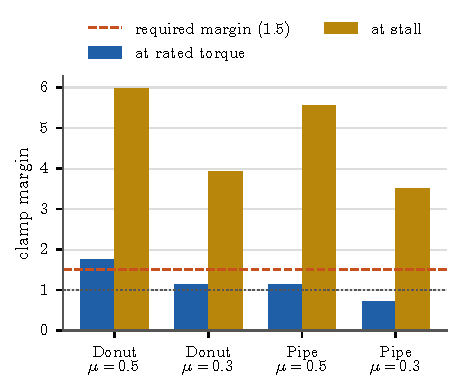
\includegraphics[width=0.48\linewidth]{fig/grip_margin.pdf}\hfill
  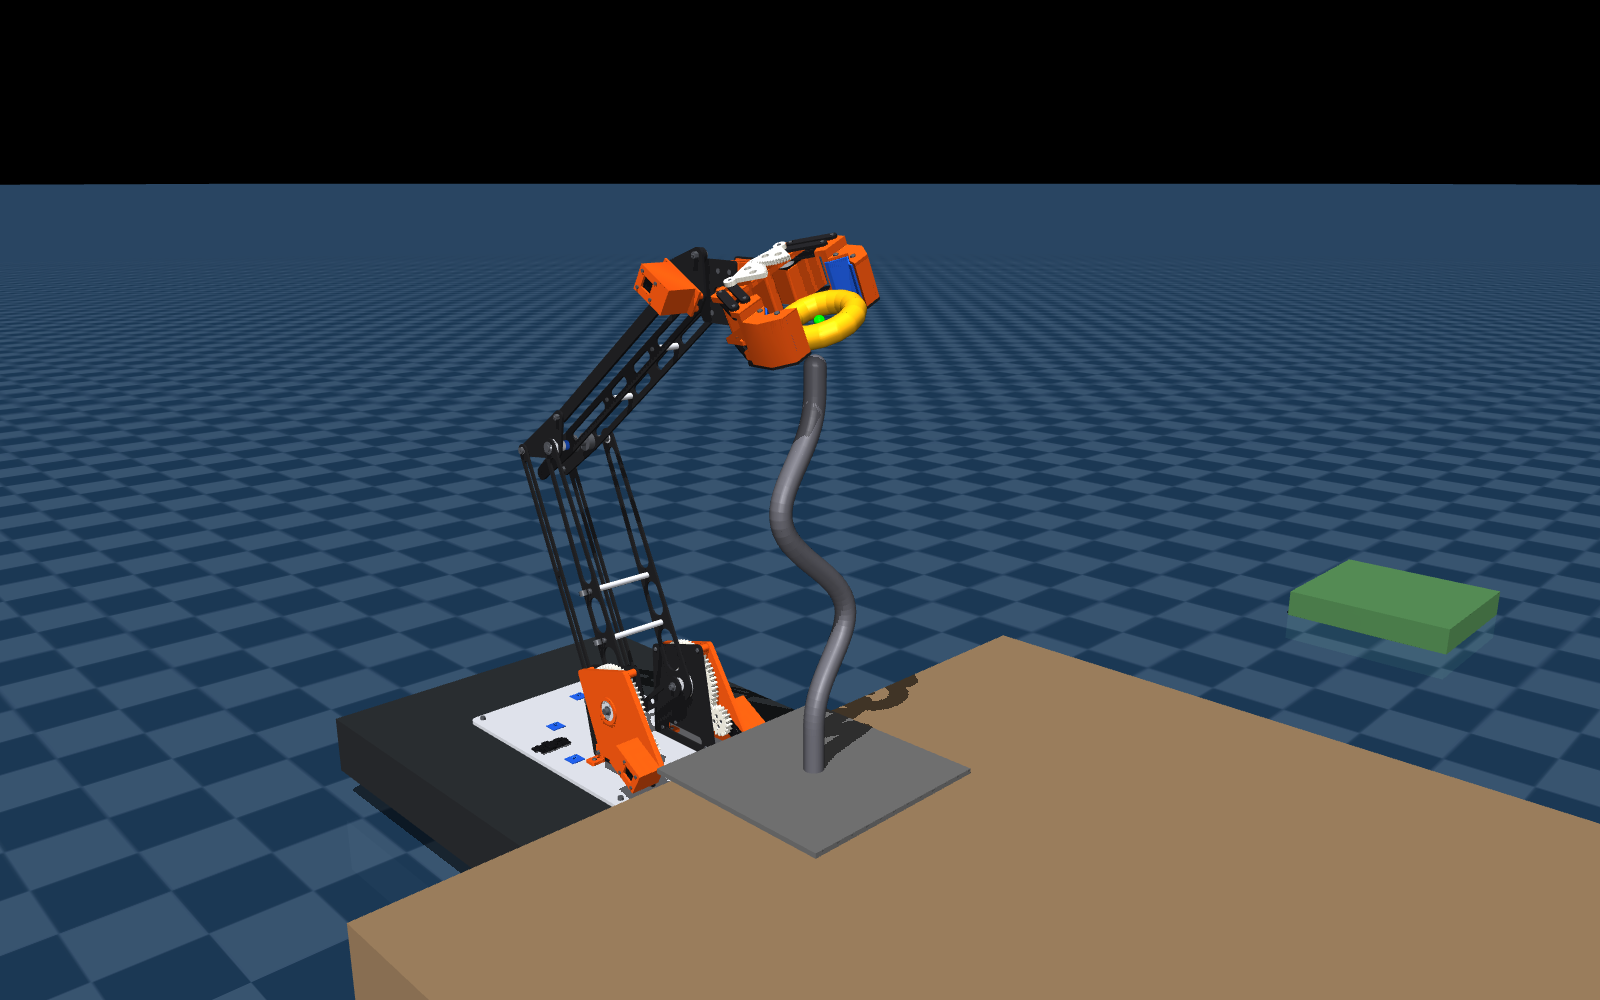
\includegraphics[width=0.48\linewidth]{fig/sim_donut_roll.png}
  \caption{Left: clamp margin for each object and pad friction, at the servo's rated and stall torque.
  Right: the donut carried up the pole with the wrist rolled (MuJoCo).}
  \label{fig:grip}
\end{figure}

\subsection{Holding torque (R4)}
The static joint torques at all 14 task poses, with the object in the jaws, are compared with each actuator's
holding limit (Fig.~\ref{fig:static}). The worst case is J1 at the donut place, \JOneTau\Nm. That is \JOneUtilG\,\% of
the geared limit and \JOneUtilD\,\% of the DM-J4340's rated torque. The wrist uses at most \JThreeUtil\,\% of its limit.

\begin{figure}[h]
  \centering
  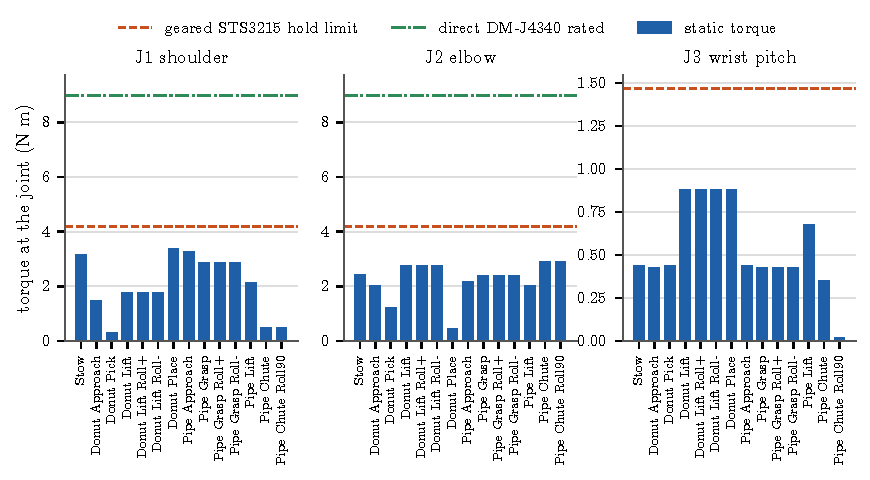
\includegraphics[width=\linewidth]{fig/static_torque.pdf}
  \caption{Static torque at each task pose against the holding limits of both base drives.}
  \label{fig:static}
\end{figure}

\subsection{Task simulation (R5)}
A MuJoCo model built from the CAD meshes runs both tasks end to end in \SimTime\,s, with position servos and
acceleration-limited moves. The donut lands flat on the platform, and the pipe ends \PipeDepth\,mm into the chute. The peak
joint torque is at most \PeakFrac\,\% of stall, and the RMS torque at most \RmsFrac\,\% of the continuous rating
(the elbow, Fig.~\ref{fig:sim}). A video of both tasks with every joint at its rated speed, played in real time, is
in the repository (\texttt{sim/media/arc\_arm\_tasks\_realtime.mp4}).

\begin{figure}[h]
  \centering
  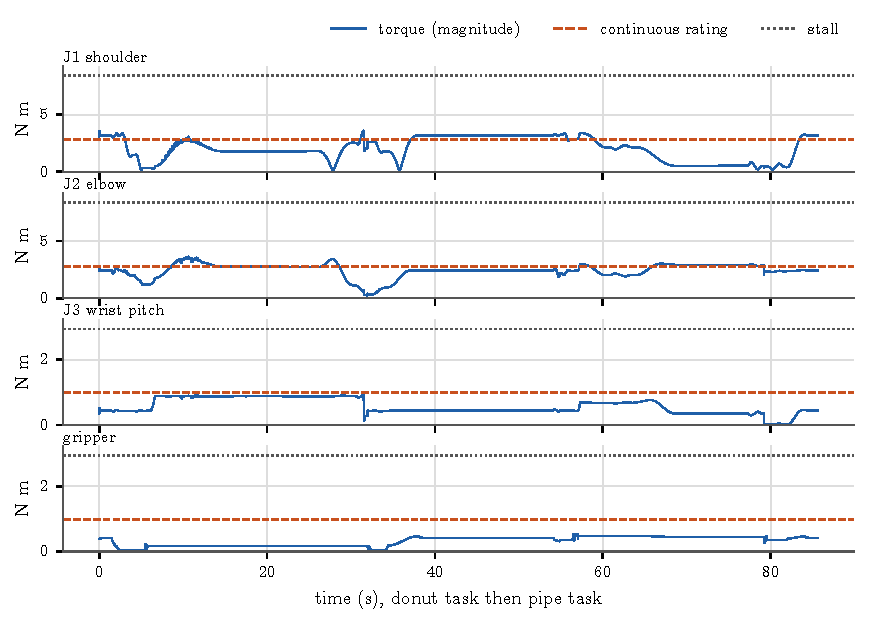
\includegraphics[width=\linewidth]{fig/sim_torque.pdf}
  \caption{Joint torque through the donut task and then the pipe task, against the continuous rating and stall.}
  \label{fig:sim}
\end{figure}

\subsection{Strength (R6)}
Every load-bearing part was analysed with second-order tetrahedral FEA (gmsh and CalculiX). Gravity and impact loads
were factored by 2.5 and actuator-limited loads by 1.25. The lowest safety factor is \MinSF, for the carbon-fibre
gripper drive link at servo stall; everything else is higher (Fig.~\ref{fig:fea}).

\begin{figure}[h]
  \centering
  \begin{minipage}[c]{0.48\linewidth}\centering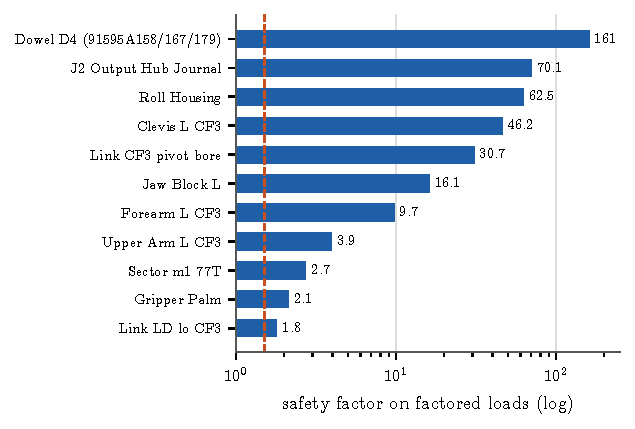
\includegraphics[width=\linewidth]{fig/fea_sf.pdf}\end{minipage}\hfill
  \begin{minipage}[c]{0.48\linewidth}\centering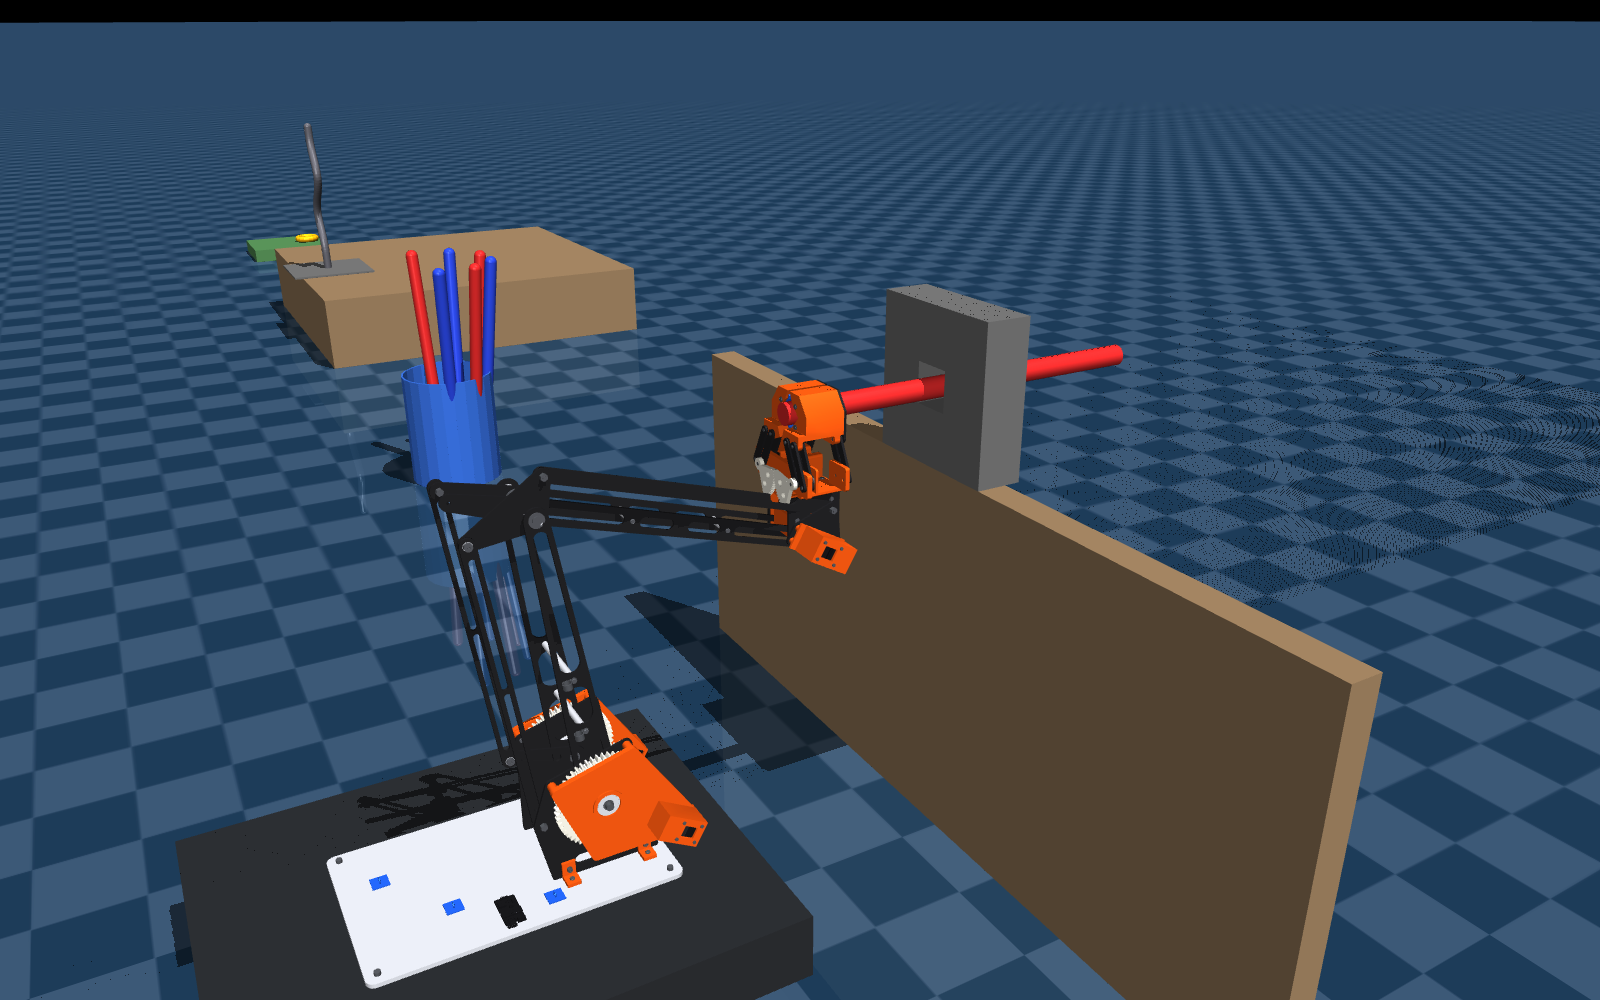
\includegraphics[width=\linewidth]{fig/sim_pipe_chute.png}\end{minipage}
  \caption{Left: safety factor of each analysed part; the dashed line is the 1.5 requirement. Right: the pipe driven
  into the chute (MuJoCo).}
  \label{fig:fea}
\end{figure}

\subsection{Collisions, keep-outs and level keeping (R7)}
A full interference check of every pair of parts found \Overlaps{} overlaps at STOW, at the 14 task poses and along
the moves between them. The arm also clears the field keep-outs at every pose and along the donut's path up the pole.
The level-keeping parallelogram closes exactly, and stays at least \DeadPoint$^\circ$ from its dead point.

\subsection{Power-off release (R8)}
In simulation the spring opens the jaws 10\,mm within \ReleaseTime\,s of power loss. The result depends on the servo's
unpowered back-drive torque, which has not been measured, so R8 stays open until the bench test.

\section{Base drive comparison}\label{sec:base}
Both revisions see the same joint torques: the base motors sit on the robot, not on the arm. The difference is
margin. The geared STS3215 holds the worst pose at \JOneUtilG\,\% of its limit and runs up to \JOneOverRated\,\% above its
continuous rating on long holds. The DM-J4340 holds the same pose at \JOneUtilD\,\% of its rated torque, with no
printed gear stage to wear or add backlash. It costs \DirectExtra\,g more at the base and
needs a 24\,V CAN bus.

\section{Design master}\label{sec:fusion}
The team designs the arm in Autodesk Fusion: a parametric assembly per revision, with a shared gripper and purchased
parts at their catalogue mass. Each Fusion version is exported to the repository as text: every part's placement,
mass and centre of mass, the joints and the parameters. The same checks then run on it. The code-CAD model that
produced the results above is the reference. At the checked versions (rev.~B v\FusionVerB, \FusionMassB\,g; rev.~A
v\FusionVerA, \FusionMassA\,g) the static joint torques agree with it within \FusionTqDiffB\,\% (rev.~B) and
\FusionTqDiffA\,\% (rev.~A) at every task pose. The interference check of the full rev.~B Fusion geometry
(\FusionSolids{} solids) finds one unintended overlap: the opening spring's rigid vendor leg touches the palm by
0.6\,mm$^3$, and that leg is bent to fit at assembly. The others are fasteners, inserts and contacts inside the vendor
servo model.

\section{Open items}
\begin{enumerate}\itemsep0pt
  \item Measure the STS3215's unpowered back-drive torque, time the power-off release with each object, and choose
  the gripper spring (R8, R2).
  \item Hold the pipe horizontal for 30\,s and log the gripper servo's temperature.
  \item Measure the rubber pad friction on PVC and on a printed donut (the margins assume 0.5).
  \item Bench-test the printed 18T/54T stage for backlash and wear, and log the J1/J2 temperature (rev.~B).
  \item Update the zig-zag pole when its drawing is published (the manual marks it TBA). The donut path is generated
  from a placeholder S-curve, so re-run the interference check.
  \item Review the Robot Building Specifications: no size or weight limit has been applied yet. The stowed arm top is
  about 420\,mm.
  \item Check on a real STS3215 that its four bottom-cap screws take the 12\,mm length and that the cradle floor
  bosses meet the case.
  \item Add a soft landing stop or gas spring: the arm falls when the robot is defeated (this is allowed by the rules).
  \item Design the chassis interface. The arm assumes a deck at 120\,mm, the shoulder 160\,mm behind the bumper, and
  4$\times$M4 into the 150$\times$160\,mm base plate.
  \item Through the 3:1 stage the J1 and J2 task ranges need more than one servo turn (Appendix~\ref{sec:servo}). Test the
  STS3215 multi-turn mode on the bench, or trim the task poses to one turn.
  \item The model has no screws that fix the gripper servo's disc horn to the lower drive link, and none that hold the
  gripper servo in its palm pocket. Add them to the model and the BOM, or confirm on the prototype that nothing is needed.
\end{enumerate}

\paragraph{Reproducibility.} The CAD model, checks, FEA and simulation are in the project repository. This document
is rebuilt from their latest results with \texttt{python -I cad/docs/paper/make\_paper.py}.

\clearpage
\appendix
\section{Build guide: printed prototype, rev.~B (servo-driven)}\label{sec:build}
This appendix takes the printed parts and the purchased hardware to a working arm in \BuildSteps{} steps. The part list,
the picture and the stack order along each joint of every step come from the CAD model
(\texttt{cad/tools/build\_guide.py}). Every one of the model's parts is assigned to exactly one step, so nothing is left
over. In the pictures, orange is what the step adds, blue is a sub-assembly built earlier on the bench, and grey is what
is already on the arm. Stacks list each part with its position along the axis at STOW, in mm.

\paragraph{Names and sides.} Parts carry the model's names (\texttt{\_L} and \texttt{\_R}). The \texttt{\_L} parts sit
at $-y$: the J1 shoulder drive, the level-keeping rods and the J3 pitch servo are all on that side.

\subsection{Prototype bill of materials}
The prototype differs from the production BOM, so it has its own: \texttt{cad/out/fourbar/print/BOM\_prototype.csv}.
\ProtoPrinted{} parts are printed. \ProtoSubst{} of them replace carbon-fibre, aluminium, steel, PTFE or shim parts,
and \ProtoHalves{} are printed in two halves and glued. The neoprene grip faces are cut from sheet. The
\ProtoBought{} purchased pieces (\ProtoBoughtLines{} kinds) are the production ones; \texttt{amazon\_buy\_list.csv}
(column \emph{prototype}) is the order. The prototype adds the consumables and tools below.
\ProtoExtras

\subsection{Prepare the parts}
\begin{enumerate}\itemsep0pt
  \item \textbf{Fits.} Use what the printed \texttt{Test\_Fit\_Small} and \texttt{Test\_Fit\_Large} pieces showed. Drill or
  ream each D4 pin bore to the size that held a pin. The pins press into one part and run freely in the other, as the
  catalogue notes for each pin say.
  \item \textbf{Glue the halves.} Dry-fit each dovetail pair (upper arms, forearms, rods). Glue it flat on glass with CA
  or epoxy, and check the end holes against the mating plate before the glue sets.
  \item \textbf{Inserts.} Set every M3 heat-set insert square and flush before assembly: the roll housing, the jaw blocks
  and the J3 cradle (see the parts table of each step).
  \item \textbf{Threads.} The production standoffs, base plate, hubs and roll hub are tapped. In the printed parts, cut
  those threads with a hand tap (M3; the M4 end of the J2 journal; the M5 ends of the J1 and J2 hubs). Don't let the
  screws form them.
  \item \textbf{Bearings.} Press each bearing square into its seat with a vice, pushing on the outer race. The steps say
  which bearing goes where. A seat that is loose in PLA takes a drop of CA on the outer race only.
  \item \textbf{Printed shafts.} The printed D10 elbow and wrist shafts carry the e-clip grooves. If a printed groove
  doesn't hold its clip, cut the shaft from the D10 steel rod (the optional buy-list line).
  \item \textbf{Shims.} Measure the printed 0.5\,mm washers and shims. Sand or reprint any that are thicker than 0.55\,mm.
  \item \textbf{Grip faces.} Cut the neoprene into strips for the R50 arc and both V flanks of each pad, and bond them with
  transfer tape. Their outer face is the grip surface (\texttt{Grip\_Rubber\_L/R}).
\end{enumerate}

\subsection{Servo setup}\label{sec:servo}
Set up each STS3215 alone on the bench before any horn goes on. Connect it to the FE-URT-1 adapter and the 12\,V
supply, and use Feetech's FD software. Give it its ID from the table, and leave the baud rate at the factory
\BusBaud. Then label the servo with its ID.
\BusTable
\noindent The horns and pinions can go on at any angle: the calibration below sets each servo's centre electronically.

\paragraph{J1 and J2 need more than one servo turn.} Through the 3:1 stage, one servo turn moves the joint 120$^\circ$.
The task poses span more than that (table). In the default position mode a servo moves within one turn, so centre J1 at
\MidJOne$^\circ$ and J2 at \MidJTwo$^\circ$, the middle of their task ranges. The poses the table lists are then out of
reach. The STS3215 also has a multi-turn mode (angle limits set to 0, about $\pm$7 turns). It doesn't keep the turn count
through a power cycle, so the arm would have to start every session at a known pose. Test that mode on the bench before
relying on it (open item).

\paragraph{Calibration, after assembly.} Move each joint to its reference angle. Then use FD's middle-position
calibration, which makes the present position read 2048, the centre.
\begin{itemize}\itemsep0pt
  \item J1 at \MidJOne$^\circ$ and J2 at \MidJTwo$^\circ$, measured with an inclinometer on the plates. J1 is the upper
  arm's angle from forward-horizontal. J2 is the forearm's absolute angle from forward-horizontal.
  \item J3 with the gripper level, and J4 with the palm level.
  \item The gripper with the jaws closed on the pipe (joint 0, the 13.8\,mm pipe grip).
\end{itemize}
Lower the torque limit in FD for the first motion tests.

\newcommand{\step}[2]{\subsection{#1}\def\steplater{\buildstep{#2}}}
\step{Base frame}{base}
Screw the four tower brackets to the base plate (tap its holes first). Then bolt the towers to the brackets with the
nyloc nuts outboard. The towers must stand square to the plate and parallel, with their hub bores in line: a D10 rod
through both bores should turn freely. Stick the two cable-tie mounts on the base plate.
\steplater

\step{Drive frames with the J1 and J2 servos (bench)}{drive_frames}
Press each 6804 into its drive-frame wall, lip outboard. Put the servo with ID~1 into the frame with the 6804 for J1, and
the servo with ID~2 into the J2 frame. Fix each servo through the cradle floor with four M2 self-tapping screws into its
own bottom-cap screw holes. Take the servo's original screws out of those holes first, and tighten the new ones only until
snug. Press the horn onto the spline and fit its centre screw. Then screw the 18T pinion to the horn with threadlocker.
\steplater

\step{Upper arm (bench)}{upper_arm}
Press a 6700 into each plate's elbow bore and the 6701 into the \texttt{\_R} plate's shoulder bore. Join the plates with the
two standoffs. Use the longer screws on the \texttt{\_L} side, where a P-clip sits under each head for the harness.
\steplater

\step{Shoulder: upper arm, J1 hub, J2 journal and crank}{shoulder}
Stand the upper arm between the towers with its shoulder bores in line with the tower bores. The hub flanges pass
through the tower bores.
\begin{itemize}\itemsep0pt
  \item \textbf{J1.} From outside the \texttt{\_L} tower, push the J1 hub in until its pilot enters the \texttt{\_L} plate.
  Fix it with three M3 screws from inside the upper arm.
  \item \textbf{J2.} From outside the \texttt{\_R} tower, push the J2 journal through the 6701. Inside, fit the crank on
  the journal's flat. Clamp it with the M4 screw and washer in the journal end.
\end{itemize}
Both hubs now turn by hand.
\steplater

\step{Base drive: gears, drive frames and end screws}{base_drive}
Slide each 54T gear onto its hub's hex until it stops on the collar. Offer each drive
frame over its hub so the journal enters the 6804 and the pinion meshes with the 54T gear. Then fit the three spacers
between frame and tower, with the M3$\times$30 screws through from the tower side and nylocs outboard. Fit the M5 screw and
washer in each hub end: they clamp the inner race against the hex shoulder. The upper arm and the crank now move only
through their servos. In the next steps, turn them with FD at a low torque limit to line up a pivot.
\steplater

\step{Forearm (bench)}{forearm}
Press a 6700 into each plate's wrist bore and join the plates with the two standoffs.
\steplater

\step{Rods (bench)}{rods}
Press an MR105 into each end of rod AB, rod 1 and rod 2.
\steplater

\step{Elbow: shaft, forearm and level rocker}{elbow}
Hold the forearm between the upper-arm plates, and put the rocker (hub with its 6700, keyed into the rocker's hex) on
the \texttt{\_L} side. Slide the elbow shaft in from the \texttt{\_L} side in the stack order below, and fit an e-clip
at each end. Tighten the two clamp collars against the inner faces of the forearm plates, so the forearm turns with the
shaft. Then check that the forearm swings freely in the upper-arm bearings, and that the rocker turns freely on the shaft.
\steplater

\step{Crank rod and level-keeping rods}{linkage}
Fit the rods in the stack orders below.
\begin{itemize}\itemsep0pt
  \item \textbf{Rod AB} joins the crank (pivot A) to the forearm (pivot B).
  \item \textbf{Rod 1} joins the \texttt{\_L} tower (G1) to the rocker (Ev1).
  \item \textbf{Rod 2} starts at the rocker (Ev2). Its far end waits for the wrist step.
\end{itemize}
Each shoulder screw's step carries a bearing's inner race, and the nyloc clamps the stack. Tighten until the stack is
firm, and check that the rod still turns freely. If the buy list's note applies (no 4\,mm shoulder screw), fit Ev1 with
the 5\,mm screw and 1.0\,mm of 5$\times$9 shims under the nut.
\steplater

\step{Clevises, roll housing and the J4 roll servo (bench)}{roll_housing}
Fix the \texttt{\_L} clevis to the roll housing with the countersunk screws, and the \texttt{\_R} clevis with button
heads. Both go into the housing's inserts. Press the 6805 into the housing. Then fix the J4 servo (ID~4) in the housing
with four M2 self-tapping screws.
\steplater

\step{Wrist level member and the J3 pitch servo (bench)}{level_member}
Press the 6700 into the wrist level hub, and key the hub into the level member's hex. Fix the J3 servo (ID~3) in its
cradle with four M2 self-tapping screws, and press its horn on. Screw the wrist-shaft coupler to the horn with the four
M3$\times$5 screws, with threadlocker. Then fix the cradle to the level member with the countersunk screws into the
cradle's inserts.
\steplater

\step{Wrist: shaft, pitch drive and rod 2}{wrist}
Set the roll housing over the forearm tip, with a clevis outside each forearm plate. Set the level member outside the
\texttt{\_L} clevis. Slide the wrist shaft in from the \texttt{\_R} side, D6 step first. It passes the \texttt{\_R}
clevis, both forearm bearings, the \texttt{\_L} clevis and the level-hub bearing, and its D6 step ends in the coupler.
Fit the e-clip outside the \texttt{\_R} clevis. Then connect rod 2 to the level member (Dv2).

Check the level keeping by hand: as the upper arm and forearm move, the level member must stay level. If it doesn't,
a rod is on the wrong hole or a hex is a flat out.
\steplater

\step{Jaws and pads (bench)}{jaws}
For each jaw, set the pad (with its neoprene) on the bottom finger plate. Thread the two D6 standoffs through the
pad. Screw the finger plate to the jaw block's wall (three screws into the wall's inserts) and to the bottom of the
standoffs; the top screws fix the standoffs to the block's top. Press the coupler pins
into the jaw block. They run in the links.
\steplater

\step{Gripper head: palm, servo, links, spring (bench)}{head}
\begin{enumerate}\itemsep0pt
  \item \textbf{Servo.} Seat the gripper servo (ID~5) in its palm pocket, and press the disc horn onto its spline.
  \item \textbf{Links.} Build the four link stacks with the jaws, using the ground pins in the stack orders below. The
  D4$\times$8 pins press into the palm from below. Fit the thrust washers either side of the ground layer.
  \item \textbf{Horn.} Screw the disc horn to the lower drive link. The model has no screws for this (open item): use
  four M3 button heads from the M3 kit, at a length that doesn't bottom in the horn.
  \item \textbf{Spring.} Fit the torsion spring on the right drive pivot, and bend and trim its legs so it opens the jaws.
\end{enumerate}
Then check by hand: the two jaws move together through the sector gears and stay parallel, the spring opens them fully,
and the servo stays in its pocket. If it lifts, hold it with a cable tie until the model gains screws.
\steplater

\step{Roll: hub and gripper head}{roll}
Slide the roll hub into the 6805 from the rear. Screw it to the J4 horn with the four M3$\times$5 screws, with
threadlocker. Then screw the gripper head's palm to the hub's front flange.
\steplater

\step{Mounting on the chassis}{chassis}
Bolt the base plate to the chassis deck with the four M4 screws.
\steplater

\subsection{Wiring and first motion}
\begin{enumerate}\itemsep0pt
  \item \textbf{Harness.} Daisy-chain the five servos on the TTL bus. Run the J3, J4 and gripper cables through the
  P-clips on the upper arm and down to the base clips. Leave a service loop at the elbow and the wrist that covers each
  joint's whole range.
  \item \textbf{Calibrate.} Power up, then calibrate each joint as in Section~\ref{sec:servo}.
  \item \textbf{One joint at a time.} Move each joint alone, slowly and at a low torque limit, from STOW through its task
  range. Watch for rubbing, the cables, and the gears skipping.
  \item \textbf{Bench tests.} Then run the open-item tests: the power-off release and the spring choice, the gear-stage
  backlash and temperature, and the J1/J2 multi-turn mode.
\end{enumerate}
Mark up this guide with whatever didn't go as written, so the next build gets it right.

\end{document}
